\newcommand{\cb}{CurryBrowser\xspace}

\section{\cb: A Tool for Analyzing and Browsing Curry Programs}
\label{sec-currybrowser}

\cb is a tool to browse through the modules and operations
of a Curry application, show them in various formats,
and analyze their properties.\footnote{Although \cb is
implemented in Curry, some functionalities of it require an
installed graph visualization tool (dot \url{http://www.graphviz.org/}),
otherwise they have no effect.}
Moreover, it is constructed in a way so that
new analyzers can easily be connected to \cb.
A detailed description of the ideas behind this tool can be
found in \cite{Hanus05WCFLP,Hanus06WLPE}.

\subsection{Installation}

The current implementation of \cb is a package
managed by the Curry Package Manager CPM
(see also Section~\ref{sec-cpm}).
Thus, to install the newest version of \cb, use the following commands:
%
\begin{curry}
> cpm update
> cpm install currybrowse
\end{curry}
%
This downloads the newest package, compiles it, and places
the executable \code{curry-browse} into the directory \code{\$HOME/.cpm/bin}.
Hence it is recommended to add this directory to your path
in order to execute \cb as described below.

\subsection{Basic Usage}

When \cb is installed as described above, it can be started in two ways:
\begin{itemize}
\item
In the \CYS environment after loading the module
\code{mod} and typing the command \ccode{:browse}.
\item
As a shell command (provided that \code{\$HOME/.cpm/bin} is
in your path): \code{curry-browse mod}
\end{itemize}
Here, \ccode{mod} is the name of the main module of a Curry application.
After the start, \cb loads the interfaces of the main
module and all imported modules before a GUI is created
for interactive browsing.

\begin{figure}[t]
\begin{center}
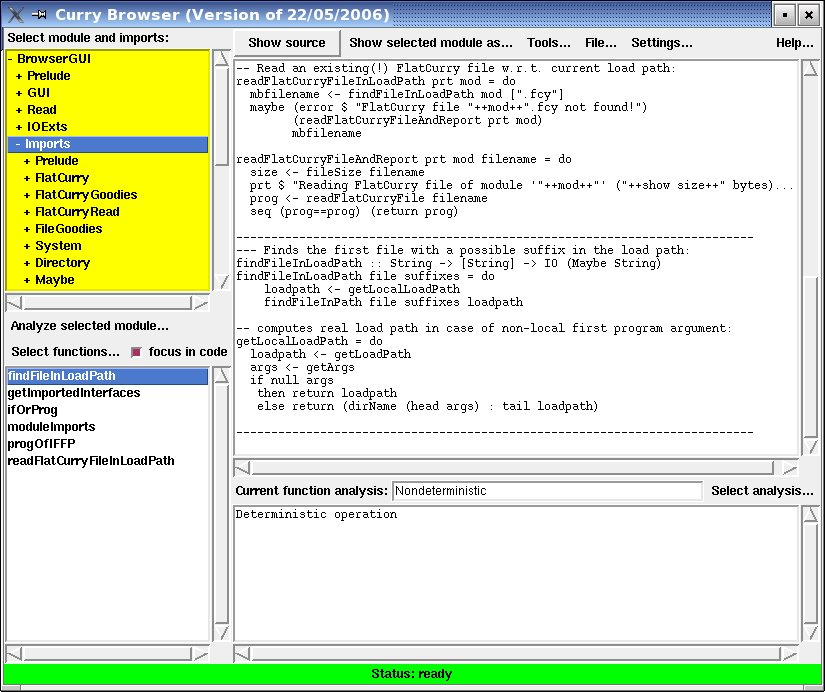
\includegraphics[scale=0.7]{tooldocs/currybrowse/currybrowser.jpg}
\end{center}
\caption{Snapshot of the main window of CurryBrowser\label{fig-currybrowser}}
\end{figure}
%
To get an impression of the use of \cb, Figure~\ref{fig-currybrowser}
shows a snapshot of its use on a particular application
(here: the implementation of \cb).
The upper list box in the left column shows the modules and their imports
in order to browse through the modules of an application.
Similarly to directory browsers, the list of imported modules of a module
can be opened or closed by clicking.
After selecting a module in the list of modules, its source code,
interface, or various other formats of the module can be shown
in the main (right) text area. For instance, one can show
pretty-printed versions of the intermediate flat programs (see below)
in order to see how local function definitions are translated by lambda lifting
\cite{Johnsson85}
or pattern matching is translated into case expressions \cite{Hanus97POPL,Wadler87}.
Since Curry is a language with parametric polymorphism and type inference,
programmers often omit the type signatures when defining functions.
Therefore, one can also view (and store) the selected module as source code where
missing type signatures are added.

Below the list box for selecting modules, there is a menu
(``Analyze selected module'') to analyze all functions
of the currently selected module at once. This is useful
to spot some functions of a module that could be problematic
in some application contexts, like functions that are impure (i.e., the result
depends on the evaluation time) or partially defined (i.e.,
not evaluable on all ground terms).
If such an analysis is selected,
the names of all functions are shown in the
lower list box of the left column (the ``function list'')
with prefixes indicating the properties of the individual functions.

The function list box can be also filled with functions
via the menu ``Select functions''. For instance, all functions
or only the exported functions defined in the currently selected
module can be shown there, or all functions from different modules
that are directly or indirectly called from
a currently selected function.
This list box is central to focus on a function in the
source code of some module or to analyze some function,
i.e., showing their properties. In order to focus on a function,
it is sufficient to check the ``focus on code'' button.
To analyze an individually selected function, one can
select an analysis from the list of available program analyses
(through the menu ``Select analysis'').
In this case, the analysis results are either shown
in the text box below the main text area
or visualized by separate tools, e.g., by a graph drawing tool for
visualizing call graphs.
Some analyses are local, i.e., they need only to consider the local definition
of this function (e.g., ``Calls directly,'' ``Overlapping rules,''
``Pattern completeness''),
where other analyses are global, i.e.,
they consider the definitions of all functions directly or indirectly called
by this function (e.g., ``Depends on,'' ``Solution complete,''
``Set-valued'').
%
Finally, there are a few additional tools integrated into \cb,
for instance, to visualize the import relation between all modules
as a dependency graph. These tools are available through the ``Tools'' menu.

More details about the use of \cb and all built-in analyses
are available through the ``Help'' menu of \cb.

